% RedlineDB system architecture diagram (camera-ready, IEEE two-column).
% Phase B sub: paper-arch. Self-contained TikZ; \input or render to EPS.
% Render: pdflatex architecture.tex && pdftops -eps architecture.pdf architecture.eps
\documentclass[crop,tikz,border=2pt]{standalone}
\usepackage{tikz}
\usepackage[T1]{fontenc}
\usepackage{helvet}
\renewcommand{\familydefault}{\sfdefault}
\usetikzlibrary{arrows.meta,positioning,fit,calc,shapes.geometric,shapes.symbols}

\begin{document}
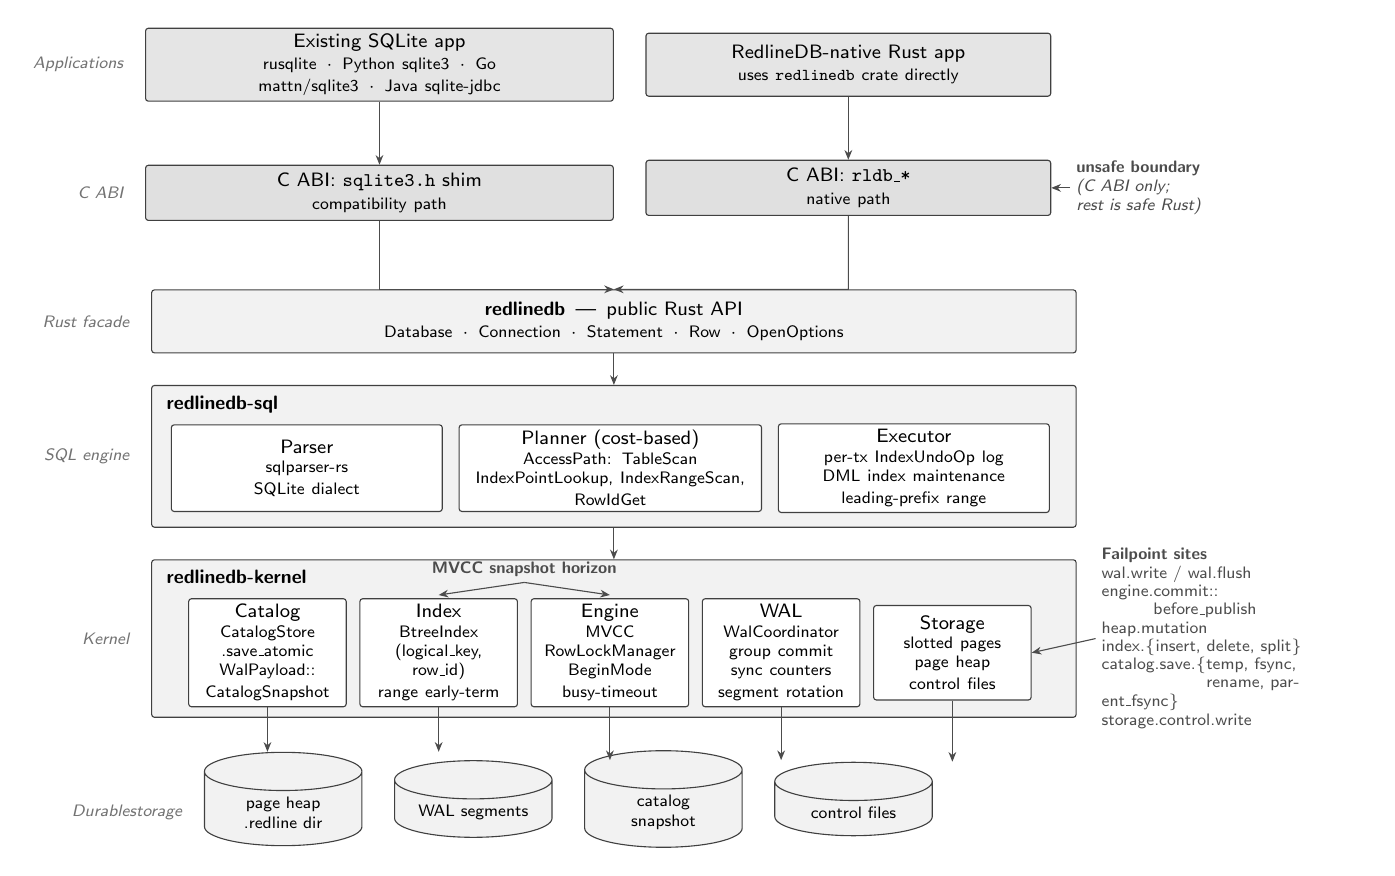
\begin{tikzpicture}[
  font=\sffamily\fontsize{7}{8}\selectfont,
  >={Stealth[length=3.5pt,width=2.8pt]},
  every node/.style={inner sep=2pt, line width=0.4pt},
  layerlbl/.style={font=\sffamily\fontsize{6}{7}\selectfont\itshape, text=black!55, anchor=west},
  box/.style={draw=black!75, line width=0.4pt, rounded corners=1pt,
              align=center, inner sep=2pt},
  layerA/.style={box, fill=black!10, minimum height=8mm},
  layerB/.style={box, fill=black!05, minimum height=8mm},
  layerC/.style={box, fill=white,    minimum height=8mm},
  abibox/.style={box, fill=black!12, minimum height=7mm},
  cell/.style={box, fill=white, minimum height=11mm, align=center,
               text width=24mm},
  kcell/.style={box, fill=white, minimum height=12mm, align=center,
                text width=18.6mm},
  cyl/.style={cylinder, draw=black!75, line width=0.4pt,
              shape border rotate=90, aspect=0.25, fill=black!05,
              minimum height=8mm, minimum width=20mm, align=center,
              text width=18mm, font=\sffamily\fontsize{6.4}{7.2}\selectfont},
  ann/.style={font=\sffamily\fontsize{6}{7}\selectfont\itshape,
              text=black!70, align=left},
  flow/.style={->, draw=black!70, line width=0.4pt},
]

% --- geometry --------------------------------------------------------------
\def\W{116mm}        % overall content width
\def\Lm{8mm}         % left margin reserved for absolutely nothing (kept tight)

% Layer 1: Applications  ----------------------------------------------------
\node[layerA, text width=58mm] (appCompat) at (0,0)
  {Existing SQLite app\\
   {\fontsize{6.2}{7}\selectfont\upshape rusqlite \,$\cdot$\, Python sqlite3 \,$\cdot$\, Go mattn/sqlite3 \,$\cdot$\, Java sqlite-jdbc}};
\node[layerA, text width=50mm, right=4mm of appCompat] (appNative)
  {RedlineDB-native Rust app\\
   {\fontsize{6.2}{7}\selectfont\upshape uses \texttt{redlinedb} crate directly}};

% Layer 2: C ABI ------------------------------------------------------------
\node[abibox, text width=58mm, below=8mm of appCompat] (abiCompat)
  {C ABI: \texttt{sqlite3.h} shim\\
   {\fontsize{6.2}{7}\selectfont\upshape compatibility path}};
\node[abibox, text width=50mm, below=8mm of appNative] (abiNative)
  {C ABI: \texttt{rldb\_*}\\
   {\fontsize{6.2}{7}\selectfont\upshape native path}};

% Layer 3: Rust facade ------------------------------------------------------
\coordinate (rowMid) at ($(abiCompat.south)!0.5!(abiNative.south)$);
\node[layerB, text width=\W, below=9mm of rowMid, anchor=north] (facade)
  {\textbf{redlinedb} \,---\, public Rust API\\
   {\fontsize{6.2}{7}\selectfont\upshape Database \,$\cdot$\, Connection \,$\cdot$\, Statement \,$\cdot$\, Row \,$\cdot$\, OpenOptions}};

% Layer 4: SQL engine -------------------------------------------------------
\node[layerB, text width=\W, below=4mm of facade, minimum height=18mm,
      align=center] (sql) {};
\node[font=\sffamily\fontsize{6.6}{7.6}\selectfont,
      anchor=north west] at ([xshift=1.2mm,yshift=-0.6mm]sql.north west)
  {\textbf{redlinedb-sql}};

\node[cell, text width=33mm] (parser) at ([xshift=-39mm,yshift=-1.5mm]sql.center)
  {Parser\\{\fontsize{6.2}{7}\selectfont sqlparser-rs\\SQLite dialect}};
\node[cell, text width=37mm, right=2mm of parser] (planner)
  {Planner (cost-based)\\
   {\fontsize{6.2}{7}\selectfont AccessPath: TableScan\\
    IndexPointLookup, IndexRangeScan,\\RowIdGet}};
\node[cell, text width=33mm, right=2mm of planner] (exec)
  {Executor\\
   {\fontsize{6.2}{7}\selectfont per-tx IndexUndoOp log\\DML index maintenance\\leading-prefix range}};

% Layer 5: Kernel -----------------------------------------------------------
\node[layerB, text width=\W, below=4mm of sql, minimum height=20mm] (kern) {};
\node[font=\sffamily\fontsize{6.6}{7.6}\selectfont,
      anchor=north west] at ([xshift=1.2mm,yshift=-0.6mm]kern.north west)
  {\textbf{redlinedb-kernel}};

\node[kcell] (kCat)  at ([xshift=-44mm,yshift=-1.8mm]kern.center)
  {Catalog\\{\fontsize{6}{7}\selectfont CatalogStore\\.save\_atomic\\
   WalPayload::\\CatalogSnapshot}};
\node[kcell, right=1.6mm of kCat] (kIdx)
  {Index\\{\fontsize{6}{7}\selectfont BtreeIndex\\(logical\_key, row\_id)\\range early-term}};
\node[kcell, right=1.6mm of kIdx] (kEng)
  {Engine\\{\fontsize{6}{7}\selectfont MVCC\\RowLockManager\\BeginMode\\busy-timeout}};
\node[kcell, right=1.6mm of kEng] (kWal)
  {WAL\\{\fontsize{6}{7}\selectfont WalCoordinator\\group commit\\sync counters\\segment rotation}};
\node[kcell, right=1.6mm of kWal] (kSto)
  {Storage\\{\fontsize{6}{7}\selectfont slotted pages\\page heap\\control files}};

% Layer 6: Durable storage --------------------------------------------------
\coordinate (kernSouth) at (kern.south);
\node[cyl] (dHeap) at ([xshift=-42mm,yshift=-12mm]kernSouth)
  {page heap\\.redline dir};
\node[cyl, right=4mm of dHeap] (dWal)  {WAL segments};
\node[cyl, right=4mm of dWal]  (dCat)  {catalog\\snapshot};
\node[cyl, right=4mm of dCat]  (dCtl)  {control files};

% Vertical flow arrows ------------------------------------------------------
\draw[flow] (appCompat.south) -- (abiCompat.north);
\draw[flow] (appNative.south) -- (abiNative.north);
\draw[flow] (abiCompat.south) -- ($(abiCompat.south)!0.5!(facade.north -| abiCompat.south)$) |- (facade.north);
\draw[flow] (abiNative.south) -- ($(abiNative.south)!0.5!(facade.north -| abiNative.south)$) |- (facade.north);
\draw[flow] (facade.south) -- (sql.north);
\draw[flow] (sql.south) -- (kern.north);

\draw[flow] (kCat.south) -- (kCat.south |- dHeap.north);
\draw[flow] (kIdx.south) -- (kIdx.south |- dHeap.north);
\draw[flow] (kEng.south) -- (kEng.south |- dWal.north);
\draw[flow] (kWal.south) -- (kWal.south |- dWal.north);
\draw[flow] (kSto.south) -- (kSto.south |- dCtl.north);

% Layer labels (left edge) --------------------------------------------------
\node[layerlbl, anchor=east] at ([xshift=-2mm]appCompat.west) {Applications};
\node[layerlbl, anchor=east] at ([xshift=-2mm]abiCompat.west) {C ABI};
\node[layerlbl, anchor=east] at ([xshift=-2mm]facade.west)    {Rust facade};
\node[layerlbl, anchor=east] at ([xshift=-2mm]sql.west)       {SQL engine};
\node[layerlbl, anchor=east] at ([xshift=-2mm]kern.west)      {Kernel};
\node[layerlbl, anchor=east] at ([xshift=-2mm]dHeap.west)     {Durable\\storage};

% --- Right-edge annotations -----------------------------------------------
% unsafe boundary -> C ABI layer only
\node[ann, anchor=west, text width=24mm] (annUnsafe)
  at ([xshift=2.4mm,yshift=0mm]abiNative.east)
  {\textbf{unsafe boundary}\\(C ABI only;\\rest is safe Rust)};
\draw[flow] (annUnsafe.west) -- (abiNative.east);

% MVCC snapshot horizon -> engine + index (placed above kernel layer)
\node[ann, anchor=south] (annMvcc)
  at ([yshift=2mm]$(kIdx.north)!0.5!(kEng.north)$)
  {\textbf{MVCC snapshot horizon}};
\draw[flow] (annMvcc.south) -- ([yshift=0.4mm]kEng.north);
\draw[flow] (annMvcc.south) -- ([yshift=0.4mm]kIdx.north);

% Failpoint sites -> WAL.write/flush, commit::before_publish, heap.mutation,
% index.{insert,delete,split}, catalog.save.{...}, storage.control.write.
% Place to the right of kernel layer.
\node[ann, anchor=west, text width=33mm] (annFail)
  at ([xshift=2.4mm]kern.east)
  {\textbf{Failpoint sites}\\
   {\fontsize{5.6}{6.6}\selectfont\upshape
    wal.write / wal.flush\\
    engine.commit::\\\hphantom{engine.}before\_publish\\
    heap.mutation\\
    index.\{insert, delete, split\}\\
    catalog.save.\{temp, fsync,\\\hphantom{catalog.save.\{}rename, parent\_fsync\}\\
    storage.control.write}};
\draw[flow] (annFail.west) -- (kSto.east);

\end{tikzpicture}
\end{document}
